\documentclass[german,a4paper]{article}

\usepackage{babel}

\usepackage{float}
\usepackage{graphicx}
\graphicspath{{fig/}}

\usepackage[utf8]{inputenc}

\title{Recommender System auf Basis von Collaborative Filtering}
\author{Alex Egger}
\date{\today}

\begin{document}

\maketitle
\newpage
\tableofcontents
\newpage

\section{Einleitung}
\textbf{Empfehlungsdienste (engl. Recommender Systems, im Folgenden RS)} sind Softwaresysteme, die zum Ziel haben, Vorhersagen über das Verhalten oder die Präferenz eines Benutzers zu treffen. Ihre Einsatzgebiete sind zahlreich und vielfältig. Ein berühmtes Beispiel stellt \textbf{Amazons Recommendation Engine} dar, welche bereits seit einigen Jahren erfolgreich im Einsatz ist. Weitere berühmte Beispiele stellen z.B. Netflix, oder MovieLense dar.
\section{Theoretischer Hintergrund}
RS sind eine Kategorie von Softwaresystemen, welche zum Oberbegriff \textbf{``Maschinelles Lernen''} gezählt werden.
\begin{quote}
\textbf{Maschinelles Lernen} ist ein Oberbegriff für die ``künstliche'' Generierung von Wissen aus Erfahrung: Ein künstliches System lernt aus Beispielen und kann nach Beendigung der Lernphase verallgemeinern. Das heißt, es werden nicht einfach die Beispiele auswendig gelernt, sondern es ``erkennt'' Gesetzmäßigkeiten in den Lerndaten. So kann das System auch unbekannte Daten beurteilen (Lerntransfer).\footnote{Von http://de.wikipedia.org/wiki/Maschinelles\_Lernen, Stand: 28.05.15}
\end{quote}
Es gibt unterschiedliche Ansätze zur Realisierung eines RS. Die drei wichtigsten Ansätze stellen folgende dar:
\begin{itemize}
\item Collabortive Filtering
\item Content-Based Filtering
\item Hybrid Recommender Systems
\end{itemize}
Im folgenden wird die Funktionsweise eines RS erklärt, welches auf Collaborative Filtering basiert.
\subsection{Collaborative Filtering}
\textbf{Collaborative Filtering (im Folgenden CF)} beschreibt den Prozess des Filterns von Informationen basierend auf der Zusammenarbeit mehrerer Datenquellen. CF-basierte Ansätze werden meist bei großen Datenmengen eingesetzt, so z.B. im Finanzbereich, oder im Bereich des E-Commerce. 
\subsubsection{Funktionsweise}
CF basiert auf der fundamentalen Annahme, dass Personen sich in ihren Vorlieben ähneln. Dies bedeutet, wenn zwei Personen ähnliche Vorlieben haben, kann man annehmen, dass dies auch in Zukunft so bleiben wird. Dieses Prinzip nutzt CF aus, um ähnliche Personen zu finden, und ihnen die Präferenzen des jeweils anderen vorzuschlagen. Desweiteren ist meist eine aktive Teilnahme des Benutzers am Quantifizierungsprozess unerlässlich. Ein typischer Aufbau eines CF-basierten Systems könnte wie folgt aussehen:
\begin{enumerate}
\item Ein Benutzer drückt seine Präferenz bezüglich eines angebotenen Objektes aus. Dies kann z.B. eine Bewertung auf einer Skala (z.B: 1 - 5), oder das Drücken eines Buttons (z.B: 0 - 1) sein.
\item Das System vergleicht die Bewertung des Benutzers mit denen der anderen Benutzer und findet jene mit den ähnlichsten Vorlieben.
\item Das System findet ein Objekt, welches ähnliche Benutzer mit einer hohen Bewertung gekennzeichnet haben und welches noch nicht vom Benutzer bewertet wurde. 
\end{enumerate}
Desweiteren existieren zwei Funktionweisen von Collaborative Filtering, die unterschiedliche Sichtpunkte auf die gegebenen Daten haben.
\\
\textbf{User-Based Collaborative Filtering (im Folgenden UBCF)} kann durch die folgenden zwei Schritte erklärt werden:
\begin{enumerate}
\item Man finde Benutzer, welche die selben Bewertungmuster haben, wie der aktuelle Benutzer.
 \item Man nutze die Bewertungen der in Schritt 1 gefundenen Benutzer, um einen Vorschlag für den aktuellen Benutzer zu berechnen.
\end{enumerate}
\textbf{Item-Based Collaborative Filtering (im Folgenden IBCF)} verhält sich ähnlich wie UBCF, aber in einer objekt-zentrischen Verhaltensweise:
\begin{enumerate}
\item Man erstelle eine Objekt-zu-Objekt-Matrix, welche Beziehungen zwischen Objektpaaren beschreibt.
\item Man erfährt die Vorlieben des aktuellen Benutzers, indem man seine Bewertungen mit der Matrix abgleicht.
\end{enumerate}
\subsubsection{Ähnlichkeit}
In \textbf{UBCF} ist es meist nötig festzustellen, wie ähnlich sich zwei Benutzer sind. Davor werden verschiedene Methoden zur Festellung der Ähnlichkeit zweier Mengen eingesetzt.
\paragraph{Euklidischer Abstand}
Der \textbf{Euklidsche Abstand} zweier Punkte in einem n-dimensionalen Raum wird wie folgt berechnet:
\begin{equation}
d(x,y) = \sqrt{\displaystyle\sum_{i=1}^{n} (x_i - y_i)^2}
\end{equation}
\paragraph{Jaccard-Index}
Eine weiter Möglichkeit besteht im \textbf{Jaccard-Index (auch Jaccard-Koeffizient}. Er ist wie folgt definiert:
\begin{equation}
J(A,B) = \frac{|A \cap B|}{|A \cup B|}
\end{equation}
\paragraph{Kosinus-Ähnlichkeit}
\textbf{Kosinus-Ähnlichkeit} ist ein Maß für die Ähnlichkeit zweier Vektoren. Sie beschreibt den Kosinus des Winkels zwischen beiden Vektoren und nimmt damit natürlich bei gleichen Vektoren den Wert 1 an. Für Vektoren die weiter von einander entfernt sind, nimmt der Wert immer weiter ab. Sie ist wie folgt definiert:
\begin{equation}
\cos(\phi) = \frac{a \cdot b}{\|a\| \cdot \|b\|} 
\end{equation}
\subsubsection{Probleme}
CF wird meist in Umgebungen mit sehr großen Datenmengen eingesetzt. Dies führt dazu, dass neue Benutzer erst genügend Bewertungen abgeben müssen, bevor für sie sinnvolle Vorhersagen getroffen werden können. Das gleiche gilt für neue Objekte, welche noch nicht genügend Bewertungen haben.\footnote{Siehe: http://en.wikipedia.org/wiki/Cold\_start} Ein weiteres Problem stellt die Skalierung von CF-basiertes System dar. Da solche Systeme oft im Web-Bereich eingesetzt werden, müssen sie sehr hohen Anforderungen an die Reaktionszeit entsprechen.
\section{Implementierung}
\subsection{Datenquellen}

\subsection{Auswahl der Filter-Methode}
Das gewählte Framework bietet verschiedene Methoden zur Filterung.
Folgende sind wählbar:
\begin{itemize}
\item \textbf{UBCF} - User-Based Collaborative Filtering
\item \textbf{IBCF} - Item-Based Collaborative Filtering
\item \textbf{POPULAR} - Filtert basierend auf der Popularität von Objekten
\item \textbf{RANDOM} - Filtert Objekte zufällig
\end{itemize}
Im Folgenden wurden die verschiedenen Ansätze bei gleichen Bedingungen und Daten eingesetzt. In Abbildung 1 ist zu sehen, wie sich die verschiedenen Methoden verhalten. \textbf{TPR (True Positive Rate)} beschreibt hier bei die Rate an Treffern, die für den Benutzer wirklich relevant sind. \textbf{FPR (False Positive Rate)} beschreibt die Rate an Treffern, die nicht relevant sind. Die Datenpunkte beschreiben dabei die Anzahl der zusuchenden Objekte. Aus Abbildung 1 kann somit abgelesen werden, dass \textbf{UBCF} sowohl die beste \textbf{TPR}, als auch die niedrigste \textbf{FPR} hat. \textbf{UBCF} wurde somit als Algorithmus zur Filterung für das RS ausgewählt.
\begin{figure}[H]
\centering
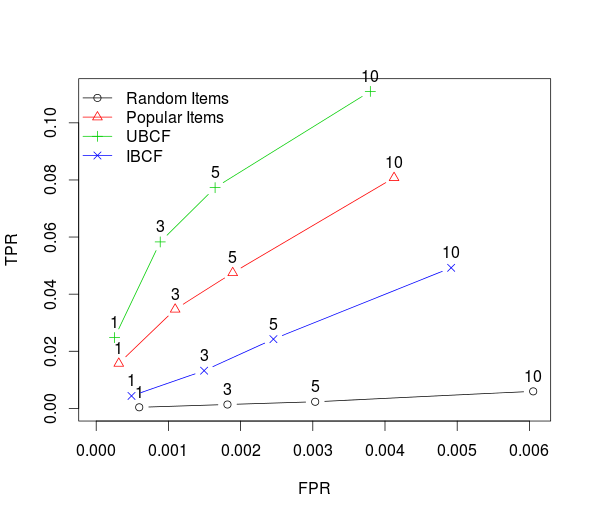
\includegraphics[width=\textwidth]{TPRFPR.png}
\caption{Vergleich der Trefferquoten verschiedener Filter-Methoden.}
\end{figure}
\section{Quellen}
\end{document}